\section*{\lr{2.3} معادل‌های منطقی}
    \begin{definition}[تعریف \lr{2.26}]
      فرض کنید $A_1, A_2 \in \mathscr{F}$. اگر برای همهٔ تعبیرها $\mathscr{I}$ داشته باشیم
      \[
      v_{\mathscr{I}}(A_1) = v_{\mathscr{I}}(A_2),
      \]
      آنگاه می‌گوییم $A_1$ \emph{معادل منطقی} $A_2$ است و با
      \[
      A_1 \equiv A_2
      \]
      نشان می‌دهیم.
    \end{definition}
      
    \begin{example}[مثال \lr{2.27}]
      آیا فرمول
      \[
      p \lor q
      \]
      معادل منطقی
      \[
      q \lor p
      \]
      است؟ چهار تعبیر متمایز برای اتم‌های $p$ و $q$ وجود دارد:
      
      \begin{center}
      \begin{tabular}{|c|c|c|c|}
      \hline
      $\mathscr{I}(p)$ & $\mathscr{I}(q)$ & $v_{\mathscr{I}}(p \lor q)$ & $v_{\mathscr{I}}(q \lor p)$ \\
      \hline
      $T$ & $T$ & $T$ & $T$ \\
      $T$ & $F$ & $T$ & $T$ \\
      $F$ & $T$ & $T$ & $T$ \\
      $F$ & $F$ & $F$ & $F$ \\
      \hline
      \end{tabular}
      \end{center}
      
      چون در همهٔ این تعبیرها صدق دو فرمول یکسان است، داریم:
      \[
      p \lor q \;\equiv\; q \lor p.
      \]
    \end{example}
      
    \begin{theorem}[قضیه \lr{2.28}]
      برای هر $A_1, A_2 \in \mathscr{F}$،
      \[
      A_1 \lor A_2 \;\equiv\; A_2 \lor A_1.
      \]
    \end{theorem}
      
    \begin{proof}
      بگذارید $\mathscr{I}$ یک تعبیر دلخواه برای $A_1 \lor A_2$ باشد. واضح است که $\mathscr{I}$ تعبیر معتبری برای $A_2 \lor A_1$ نیز هست، زیرا:
      \[
      \mathscr{P}_{A_1} \cup \mathscr{P}_{A_2} \;=\; \mathscr{P}_{A_2} \cup \mathscr{P}_{A_1}.
      \]
      
      از آنجا که $\mathscr{P}_{A_1} \subseteq \mathscr{P}_{A_1} \cup \mathscr{P}_{A_2}$، تعبیر $\mathscr{I}$ به همهٔ اتم‌های $A_1$ مقدار می‌دهد و بنابراین تعبیر معتبری برای $A_1$ است؛ به‌طور مشابه برای $A_2$.
      
      اکنون داریم:
      \[
      v_{\mathscr{I}}(A_1 \lor A_2) = T
      \;\Longleftrightarrow\;
      v_{\mathscr{I}}(A_1) = T \;\lor\; v_{\mathscr{I}}(A_2) = T,
      \]
      و
      \[
      v_{\mathscr{I}}(A_2 \lor A_1) = T
      \;\Longleftrightarrow\;
      v_{\mathscr{I}}(A_2) = T \;\lor\; v_{\mathscr{I}}(A_1) = T.
      \]
      
      اگر $v_{\mathscr{I}}(A_1) = T$، آن‌گاه
      \[
      v_{\mathscr{I}}(A_1 \lor A_2) = T = v_{\mathscr{I}}(A_2 \lor A_1),
      \]
      و همین‌طور اگر $v_{\mathscr{I}}(A_2) = T$.
      
      چون $\mathscr{I}$ دلخواه بود، نتیجه می‌گیریم:
      \[
      A_1 \lor A_2 \equiv A_2 \lor A_1.
      \]
    \end{proof}

\subsection*{\lr{2.3.1} \quad (رابطهٔ بین \lr{$\leftrightarrow$} و \lr{$\equiv$})}
    عملگر «معادل» (\lr{$\leftrightarrow$}) یک \emph{عملگر بولی} در منطق گزاره‌ای است و می‌تواند در فرمول‌های این منطق ظاهر شود. اما «معادل منطقی» (\lr{$\equiv$}) یک عملگر بولی نیست؛ بلکه نشانه‌ای برای ویژگی یک جفت فرمول در منطق گزاره‌ای است. این دو مفهوم می‌توانند سردرگمی ایجاد کنند، زیرا ما از واژگان مشابه هم برای زبان مَحْتوایی (در اینجا زبان منطق گزاره‌ای) و هم برای زبان مَدرِکی—آنچه برای استدلال دربارهٔ زبان محتوا استفاده می‌کنیم—بهره می‌بریم.
    
    با این حال، معادل بودن (\lr{$\leftrightarrow$}) و معادل منطقی (\lr{$\equiv$}) ارتباط نزدیکی دارند، چنان‌که در قضیهٔ زیر نشان داده شده است:
    
    \begin{theorem}[قضیه \lr{2.29}]
      $A_1 \equiv A_2$ اگر و تنها اگر $A_1 \leftrightarrow A_2$ در هر تعبیر صدق کند.
    \end{theorem}
    
    \begin{proof}
      فرض کنید $A_1 \equiv A_2$ و $\mathscr{I}$ یک تعبیر دلخواه باشد. از تعریف معادل منطقی می‌دانیم:
      \[
      v_{\mathscr{I}}(A_1) = v_{\mathscr{I}}(A_2).
      \]
      طبق جدول ارزش صدق (شکل \lr{2.3})، در این صورت داریم:
      \[
      v_{\mathscr{I}}(A_1 \leftrightarrow A_2) = T.
      \]
      از آنجا که $\mathscr{I}$ دلخواه بود، نتیجه می‌شود $A_1 \leftrightarrow A_2$ در همهٔ تعبیرها درست است.
      
      اثبات جهت معکوس (یعنی اگر $A_1 \leftrightarrow A_2$ در همهٔ تعبیرها درست باشد، آنگاه $A_1 \equiv A_2$) به‌صورتی مشابه انجام می‌پذیرد.
    \end{proof}
    
    \begin{figure}[ht]
      \centering
      \begin{latin}
      \resizebox{0.7\textwidth}{!}{
      \begin{tikzpicture}[
        level distance=1.5cm,
        sibling distance=4cm,
        level 2/.style={sibling distance=2cm},
        level 3/.style={sibling distance=1cm},
        edge from parent path={(\tikzparentnode.south) -- (\tikzchildnode.north)}
      ]
      \node {$\leftrightarrow$}
        child { 
          node {$\rightarrow$}
          child {node {$p$}}
          child {node {$p$}}
        }
        child { 
          node {$\rightarrow$}
          child {
            node {$\neg$}
            child {node {$p$}}
          }
          child {
            node {$\neg$}
            child {node {$q$}}
          }
        };
      \end{tikzpicture}
      }
      \\
      \resizebox{0.2\textwidth}{!}{
        \begin{tikzpicture}[
          level distance=0.75cm,
          sibling distance=0.75cm,
          level 2/.style={sibling distance=1cm},
          edge from parent path={(\tikzparentnode.south) -- (\tikzchildnode.north)}
        ]
        \node {$\rightarrow$}
          child { 
            child {node {$p$}}
            child {node {$p$}}
          };
        \end{tikzpicture}
      }
      \hfill
      \resizebox{0.1\textwidth}{!}{
        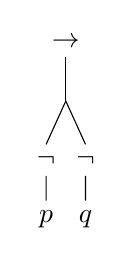
\begin{tikzpicture}[
          level distance=0.75cm,
          sibling distance=0.75cm,
          level 2/.style={sibling distance=0.5cm},
          level 3/.style={sibling distance=0.5cm},
          edge from parent path={(\tikzparentnode.south) -- (\tikzchildnode.north)}
        ]
        \node {$\rightarrow$}
          child { 
            child {
              node {$\neg$}
              child {node {$p$}}
            }
            child {
              node {$\neg$}
              child {node {$q$}}
            }
          };
        \end{tikzpicture}
      }
      \hfill
      \resizebox{0.1\textwidth}{!}{
        \begin{tikzpicture}[
          level distance=0.75cm,
          sibling distance=0.75cm,
          level 2/.style={sibling distance=0.5cm},
          level 3/.style={sibling distance=0.5cm},
          edge from parent path={(\tikzparentnode.south) -- (\tikzchildnode.north)}
        ]
        \node {$\neg$}
          child { 
            child { node {$p$} }
          };
          
        \end{tikzpicture}
      }
      \hfill
      \resizebox{0.1\textwidth}{!}{
        \begin{tikzpicture}[
          level distance=0.75cm,
          sibling distance=0.75cm,
          level 2/.style={sibling distance=0.5cm},
          level 3/.style={sibling distance=0.5cm},
          edge from parent path={(\tikzparentnode.south) -- (\tikzchildnode.north)}
        ]
        \node {$\neg$}
          child { 
            child { node {$q$} }
          };
          
        \end{tikzpicture}
      }
      \hfill
      \resizebox{0.1\textwidth}{!}{
        \begin{tikzpicture}[
          level distance=0.75cm,
          sibling distance=0.75cm,
          level 2/.style={sibling distance=0.5cm},
          level 3/.style={sibling distance=0.5cm},
          edge from parent path={(\tikzparentnode.south) -- (\tikzchildnode.north)}
        ]
        \node {$p$};
          
        \end{tikzpicture}
      }
      \hfill
      \resizebox{0.1\textwidth}{!}{
        \begin{tikzpicture}[
          level distance=0.75cm,
          sibling distance=0.75cm,
          level 2/.style={sibling distance=0.5cm},
          level 3/.style={sibling distance=0.5cm},
          edge from parent path={(\tikzparentnode.south) -- (\tikzchildnode.north)}
        ]
        \node {$q$};
          
        \end{tikzpicture}
      }
      \end{latin}
      \renewcommand{\thefigure}{\lr{2.4}}
      \caption{زیر فرمول ها}
      \end{figure}
\subsection*{\lr{2.3.2} جایگزینی}
      معادل منطقی توجیه‌کنندهٔ جایگزینی یک فرمول به‌جای فرمول دیگری است.
      
      \begin{definition}[تعریف \lr{2.30}]
        اگر $A$ زیردرختی از فرمول $B$ باشد، آنگاه می‌گوییم $A$ یک \emph{زیرفرمول} از $B$ است. اگر $A$ دقیقاً با $B$ یکسان نباشد، آن را \emph{زیرفرمول درست} $B$ می‌نامیم.
      \end{definition}
      
      \begin{example}[مثال \lr{2.31}]
        شکل \lr{2.4} فرمول
        \[
        (p \to q) \;\leftrightarrow\; (\neg p \to \neg q)
        \]
        (فرمول سمت چپ شکل \lr{2.1}) و زیرفرمول‌های درست آن را نشان می‌دهد.
        اگر به‌صورت رشته نمایش داده شود، زیرفرمول‌های درست عبارتند از:
        \[
        p \to q,\quad \neg p \to \neg q,\quad \neg p,\quad \neg q,\quad p,\quad q.
        \]
      \end{example}
      
      \begin{definition}[تعریف \lr{2.32}]
        فرض کنید $A$ یک زیرفرمول از $B$ باشد و $A'$ هر فرمول دلخواهی باشد.
        $B\{A \leftarrow A'\}$ یعنی جایگزینی $A'$ به‌جای $A$ در $B$، فرمولی است که از $B$ به‌دست می‌آید وقتی همهٔ زیردرخت‌های متناظر با $A$ در $B$ با $A'$ جایگزین شوند.
      \end{definition}
      
      \begin{example}[مثال \lr{2.33}]
        بگذارید
        \[
        B = (p \to q) \leftrightarrow (\neg p \to \neg q),\quad
        A = p \to q,\quad
        A' = \neg p \lor q.
        \]
        آنگاه
        \[
        B\{A \leftarrow A'\}
        \;=\;
        (\neg p \lor q) \;\leftrightarrow\; (\neg q \to \neg p).
        \]
      \end{example}
      
      اگر در فرمول $B$، یک زیرفرمول $A$ با فرمولی که معادل منطقی $A$ است جایگزین شود، ارزش‌گذاری $B$ در هیچ تعبیر تغییر نمی‌کند.
      
      \begin{theorem}[قضیه \lr{2.34}]
        فرض کنید $A$ زیرفرمولی از $B$ باشد و $A'$ فرمولی باشد که $A \equiv A'$. آنگاه
        \[
        B \;\equiv\; B\{A \leftarrow A'\}.
        \]
      \end{theorem}
      
      \begin{proof}
        بگذارید $\mathscr{I}$ یک تعبیر دلخواه باشد. چون $A \equiv A'$، پس:
        \[
        v_{\mathscr{I}}(A) = v_{\mathscr{I}}(A').
        \]
        باید نشان دهیم:
        \[
        v_{\mathscr{I}}(B)
        =
        v_{\mathscr{I}}\bigl(B\{A \leftarrow A'\}\bigr).
        \]
        اثبات با استقرا بر عمق $d$ بالاترین وقوع زیردرخت $A$ در $B$ انجام می‌شود:
        
        \begin{itemize}
          \item \textbf{حالت پایه} ($d = 0$):  
            در این حالت، تنها یک وقوع از $A$ وجود دارد که همان خود $B$ است. پس:
            \[
            v_{\mathscr{I}}(B)
            = v_{\mathscr{I}}(A)
            = v_{\mathscr{I}}(A')
            = v_{\mathscr{I}}\bigl(B\{A \leftarrow A'\}\bigr).
            \]
          \item \textbf{گام استقرا} ($d > 0$):  
            در این حالت، $B$ یکی از دو صورت زیر است:
            \begin{enumerate}
              \item $B = \neg B_1$,
              \item $B = B_1\;\mathrm{op}\;B_2$ برای برخی فرمول‌های $B_1, B_2$ و یک عملگر بولی $\mathrm{op}$.
            \end{enumerate}
            در هر دو صورت، عمق $A$ در زیردرخت‌های $B_1$ و $B_2$ کمتر از $d$ است. بنابراین، بر اساس فرض استقرا:
            \[
            v_{\mathscr{I}}(B_1)
            = v_{\mathscr{I}}\bigl(B_1\{A \leftarrow A'\}\bigr),
            \quad
            v_{\mathscr{I}}(B_2)
            = v_{\mathscr{I}}\bigl(B_2\{A \leftarrow A'\}\bigr).
            \]
            پس بر اساس تعریف ارزش‌گذاری برای عملگرهای بولی:
            \[
            v_{\mathscr{I}}(B)
            = v_{\mathscr{I}}\bigl(B\{A \leftarrow A'\}\bigr).
            \]
        \end{itemize}
        در نتیجه، از آنجا که $\mathscr{I}$ دلخواه بود داریم:
        \[
        B \equiv B\{A \leftarrow A'\}.
        \]
      \end{proof}
\subsection*{\lr{2.3.3}  فرمول‌های معادل منطقی}
      جایگزینی فرمول‌های معادل منطقی اغلب انجام می‌شود، برای مثال در ساده‌سازی فرمول‌ها، و آشنایی با معادل‌های پرکاربرد فهرست‌شده در این زیربخش ضروری است. اثبات آن‌ها از تعاریف ابتدایی به‌دست می‌آید و به‌عنوان تمرین باقی گذاشته شده است.
      
      \subsubsection*{جذب ثابت‌ها \lr{(Absorption of Constants)}}
      اجازه دهید نحو فرمول‌های بولی را طوری گسترش دهیم که دو گزارهٔ اتمی ثابت \(\text{true}\) و \(\text{false}\) را نیز شامل شود. (نمادهای دیگر: \(\top\) برای \(\text{true}\) و \(\bot\) برای \(\text{false}\).) معنای آن‌ها به صورت زیر تعریف می‌شود:
      \[
      \mathscr{I}(\text{true}) = T
      \quad\text{و}\quad
      \mathscr{I}(\text{false}) = F
      \]
      برای هر تعبیر \(\mathscr{I}\).  
      این نمادها را نباید با مقادیر صدق \(T\) و \(F\) که در تعریف ارزش‌گذاری به‌کار می‌روند، اشتباه گرفت. همچنین می‌توان \(\text{true}\) و \(\text{false}\) را به‌ترتیب به‌عنوان اختصار برای فرمول‌های زیر در نظر گرفت:
      \[
      p \lor \neg p
      \quad\text{و}\quad
      p \land \neg p.
      \]
      وقوع یک ثابت در فرمول ممکن است آن را چنان فرو بکاهد که عملگر دودویی بی‌نیاز شود یا حتی فرمول به یک ثابت تبدیل شود:
      \[
      \begin{aligned}
      A \lor \text{true} &\equiv \text{true}
      &\quad
      A \land \text{true} &\equiv A\\
      A \lor \text{false} &\equiv A
      &\quad
      A \land \text{false} &\equiv \text{false}\\
      A \to \text{true} &\equiv \text{true}
      &\quad
      \text{true} \to A &\equiv A\\
      A \to \text{false} &\equiv \neg A
      &\quad
      \text{false} \to A &\equiv \text{true}\\
      A \leftrightarrow \text{true} &\equiv A
      &\quad
      A \oplus \text{true} &\equiv \neg A\\
      A \leftrightarrow \text{false} &\equiv \neg A
      &\quad
      A \oplus \text{false} &\equiv A
      \end{aligned}
      \]
      
      \subsubsection*{عملوندهای همسان \lr{(Identical Operands)}}
      فروپاشی (collapse) همچنین وقتی رخ می‌دهد که هر دو عملوند یکسان باشند یا یکی نقیض دیگری:
      \[
      \begin{aligned}
      A &\equiv \neg\neg A,\\
      A &\equiv A \land A
      &\quad
      A &\equiv A \lor A,\\
      A \lor \neg A &\equiv \text{true}
      &\quad
      A \land \neg A &\equiv \text{false},\\
      A \to A &\equiv \text{true},\\
      A \leftrightarrow A &\equiv \text{true}
      &\quad
      A \oplus A &\equiv \text{false},\\
      \neg A &\equiv A \uparrow A
      &\quad
      \neg A &\equiv A \downarrow A.
      \end{aligned}
      \]
      
      \subsubsection*{جابجایی، پیمایش‌پذیری، و توزیع‌پذیری}
      اپراتورهای دودویی بولی—به‌جز «تضمین» (\(\to\))—هم جابجایی‌پذیرند و هم پیمایش‌پذیر:
      \[
      \begin{aligned}
      A \lor B &\equiv B \lor A
      &\quad
      A \land B &\equiv B \land A,\\
      A \leftrightarrow B &\equiv B \leftrightarrow A
      &\quad
      A \oplus B &\equiv B \oplus A,\\
      A \uparrow B &\equiv B \uparrow A
      &\quad
      A \downarrow B &\equiv B \downarrow A.
      \end{aligned}
      \]
      با ورود نقیض، جهت یک تضمین می‌تواند وارونه شود:
      \[
      A \to B \;\equiv\; \neg B \to \neg A.
      \]
      فرمول \(\neg B \to \neg A\) را \emph{مخالف‌مقدم} (contrapositive) \(\,A \to B\) می‌نامند.
      
      جمع‌گزاره (\(\lor\))، ضرب‌گزاره (\(\land\))، معادل (\(\leftrightarrow\)) و نامعادل (\(\oplus\)) پیمایش‌پذیرند:
      \[
      \begin{aligned}
      A \lor (B \lor C) &\equiv (A \lor B) \lor C
      &\quad
      A \land (B \land C) &\equiv (A \land B) \land C,\\
      A \leftrightarrow (B \leftrightarrow C) &\equiv (A \leftrightarrow B) \leftrightarrow C
      &\quad
      A \oplus (B \oplus C) &\equiv (A \oplus B) \oplus C.
      \end{aligned}
      \]
      ولی تضمین (\(\to\))، nor (\(\downarrow\)) و nand (\(\uparrow\)) پیمایش‌پذیر نیستند.
      
      همچنین، جمع‌گزاره و ضرب‌گزاره بر یکدیگر توزیع‌پذیرند:
      \[
      \begin{aligned}
      A \lor (B \land C) &\equiv (A \lor B) \land (A \lor C),\\
      A \land (B \lor C) &\equiv (A \land B) \lor (A \land C).
      \end{aligned}
      \]
      
      \subsubsection*{تعریف یک عملگر به‌واسطهٔ عملگر دیگر}
      در اثبات قضایا با استقرا ساختاری، گام استقرایی باید برای هر عملگر دودویی جداگانه انجام شود. این گام‌ها ساده‌تر می‌شوند اگر بتوان عملگرهای خاص را با جایگزینی زیرفرمول‌هایی حذف کرد و فقط از مجموعه‌ای از عملگرهای پایه بهره گرفت. مثلاً معادل (\(\leftrightarrow\)) را می‌توان با ترکیب تضمین و ضرب‌گزاره تعریف کرد.
      
      همچنین، برخی الگوریتم‌ها برای تبدیل فرمول به شکل نرمال، نیازمند حذف برخی عملگرها هستند. فهرست معادل‌هایی که برای این کار کاربرد دارند:
      \[
      \begin{aligned}
      A \leftrightarrow B &\equiv (A \to B) \land (B \to A)
      &\quad
      A \oplus B &\equiv \neg(A \to B) \lor \neg(B \to A),\\
      A \to B &\equiv \neg A \lor B
      &\quad
      A \to B &\equiv \neg(A \land \neg B),\\
      A \lor B &\equiv \neg(\neg A \land \neg B)
      &\quad
      A \land B &\equiv \neg(\neg A \lor \neg B),\\
      A \lor B &\equiv \neg A \to B
      &\quad
      A \land B &\equiv \neg(A \to \neg B).
      \end{aligned}
      \]
      تعریف ضرب‌گزاره برحسب جمع‌گزاره و نقیض و بالعکس را \emph{قضایای دمورگان} \lr{(De Morgan’s laws)} می‌نامند.